\documentclass[final]{beamer}

\usepackage[T1]{fontenc}
\usepackage{lmodern}
\usepackage[orientation=portrait,size=a0,scale=1.0]{beamerposter}
\usetheme{gemini}
\usecolortheme{nott}
\usepackage{graphicx}
\usepackage{booktabs}
\usepackage{tikz}
\usepackage{pgfplots}
\pgfplotsset{compat=1.14}
\usepackage{anyfontsize}
\usepackage[spanish]{babel}
\usepackage[utf8]{inputenc}
\usepackage{graphicx}
\usepackage[labelfont=bf]{caption}
% Operadores matemáticos:
\DeclareMathOperator*{\argmin}{arg\,min}
\DeclareMathOperator*{\argmax}{arg\,max}
\DeclareMathOperator*{\essinf}{ess\,inf}

% Conjuntos y espacios:
\newcommand{\R}{\mathbb{R}}
\newcommand{\N}{\mathbb{N}}
\newcommand{\xspace}{\mathcal{X}}
\newcommand{\yspace}{\mathcal{Y}}
\newcommand{\salgebra}{\mathcal{S}}
\newcommand{\borel}[1]{\mathcal{B}\parent{#1}}
\newcommand{\matrixspace}[2]{\mathcal{M}_{#1}\parent{#2}}
\newcommand{\power}[1]{\mathcal{P}\parent{#1}}
\newcommand{\supp}[1]{\operatorname{Supp}\parent{#1}}
\newcommand{\lspace}[2]{\operatorname{L}^{#1}\parent{#2}}
\newcommand{\continuous}[1]{\mathcal{C}\parent{#1}}
\newcommand{\continuousb}[1]{\mathcal{C}_b\parent{#1}}
\newcommand{\posmeasure}[1]{\mathcal{M}_+\parent{#1}}
\newcommand{\probmeasure}[1]{\mathcal{M}_+^1\parent{#1}}
\newcommand{\probmeasurep}[1]{\mathcal{M}_+^{1,p}\parent{#1}}
\newcommand{\cone}[1]{\R^{#1}_{++}/_\sim}

% Funciones y operadores:
\newcommand{\parent}[1]{\left(#1\right)}
\newcommand{\rparent}[1]{\left[#1\right]}
\newcommand{\norm}[1]{\left\lVert #1 \right\rVert}
\newcommand{\dotproduct}[2]{\left\langle #1,\,#2\right\rangle}
\newcommand{\trace}[1]{\operatorname{Tr}\parent{#1}}
\newcommand{\diag}[1]{\operatorname{diag}\parent{#1}}
\newcommand{\score}[2]{\nabla_{#1} \log #2}
\newcommand{\identity}[1]{\operatorname{I}_{#1}}
\newcommand{\1}{\mathds{1}}
\newcommand{\wasserstein}[2]{\mathcal{W}_{#1}\parent{#2}}
\newcommand{\weak}{\rightharpoonup}
\newcommand{\hmetric}[2]{d_{\mathcal{H}}\parent{#1,#2}}
\renewcommand{\d}{\,\operatorname{d}\!}

% Probabilidades:
\newcommand{\E}[2]{\mathbb{E}_{#1}\rparent{#2}}
\newcommand{\var}[1]{\operatorname{Var}\parent{#1}}
\newcommand{\cov}[2]{\operatorname{Cov}\parent{#1,\,#2}}
\newcommand{\ley}[1]{\operatorname{Ley}\parent{#1}}
\newcommand{\gaussian}[2]{\mathcal{N}\parent{#1,\,#2}}

% Teoría de la información:
\newcommand{\KL}[2]{\operatorname{D_{KL}}\parent{#1\,\|\,#2}}
\newcommand{\fdiv}[2]{\operatorname{D}_f\parent{#1\,\|\,#2}}
\newcommand{\TV}[2]{\operatorname{D_{TV}}\parent{#1\,\|\,#2}}
\newcommand{\DF}[2]{\operatorname{D_F}\parent{#1\,\|\,#2}}
\newcommand{\entropy}[1]{\mathcal{H}\parent{#1}}
\newcommand{\elbo}{\operatorname{ELBO}}

% Otros:
\newcommand{\feasible}[2]{\genfrac {}{}{0pt}{2}{#1}{#2}}
\newcommand{\cte}{\operatorname{constante}}
\newcommand{\gibbs}{\mathcal{K}}
\newcommand{\ptrue}{p_{\operatorname{true}}}
\newcommand{\pprior}{p_{\operatorname{prior}}}

% Imágenes:
\newcommand{\insertimage}[3]{
    \begin{figure}
        \centering
        \includegraphics[width=#2\textwidth]{./images/#1}
        \caption{#3}
        \label{fig:#1}
    \end{figure}
}

% Temporal:
\newcommand{\pendiente}[1]{\colorbox{yellow}{#1}}

\newlength{\sepwidth}
\newlength{\colwidth}
\setlength{\sepwidth}{0.025\paperwidth}
\setlength{\colwidth}{0.45\paperwidth}

\newcommand{\separatorcolumn}{\begin{column}{\sepwidth}\end{column}}

\title{Modelos de difusión, transporte óptimo y puentes de Schrödinger}

\author{Fernando Fêtis Riquelme}

\institute[shortinst]{DIM/MDS - Universidad de Chile}

\footercontent{
  \href{https://github.com/fernando-fetis/tesis}{https://github.com/fernando-fetis/tesis} \hfill
  Jornada Técnica AC3E 2024 - Universidad Técnica Federico Santa María\hfill
  \href{mailto:fernando.fetis@uchile.cl}{fernando.fetis@uchile.cl}}

\logoright{\includegraphics[height=7cm,opacity=0.5]{logos/ac3e}}
\logoleft{\includegraphics[height=7cm,opacity=0.5]{logos/fcfm}}

\begin{document}

\begin{frame}[t]
  \begin{columns}[t]
    \separatorcolumn

    \begin{column}{\colwidth}

      \begin{block}{Formulación de los modelos de difusión}
        Los modelos de difusión son una familia de \textbf{modelos generativos} que buscan aprender a generar muestras a partir de una distribución de datos $\ptrue$. Para esto, realizan un proceso de distorsión \eqref{eq:ddpm_forward} sobre muestras de $\ptrue$, transformándolas en muestras de otra distribución $\pprior$. En paralelo, una red neuronal $p_\theta$ busca aprender el proceso de reconstrucción mediante \eqref{eq:ddpm_backward}.

        \heading{Procesos de difusión y reconstrucción}

        Dada una secuencia de ruidos, $(\beta_t)_{t=1}^T$, el proceso de difusión es una cadena de Markov que progresivamente va inyectando ruido gaussiano a muestras $x_0\sim q(x_0)=\ptrue(x_0)$ hasta llegar a una muestra final $x_T\sim q(x_T)\approx\pprior(x_T)$ mediante el proceso forward con factorización causal

        \begin{equation}
          \label{eq:ddpm_forward}
          q(x_{1:T}|x_0) = \prod_{t=1}^{T} q(x_t|x_{t-1}),
          \quad\text{donde}\quad
          q(x_t|x_{t-1}) \sim \gaussian{\sqrt{1-\beta}\, x_{t-1}}{\beta_t\identity{d}}
        \end{equation}

        El proceso de reconstrucción es otra cadena de Markov (hacia atrás en el tiempo) que busca aprender las transiciones reversas $q(x_{t-1}|x_t)$ mediante un modelo paramétrico $p_\theta(x_{t-1}|x_t)$. Este proceso es el que permite generar nuevas muestras comenzando desde $x_T$:

        \begin{equation}
          \label{eq:ddpm_backward}
          p_\theta(x_{0:T}) = p_\theta(x_T)\prod_{t=1}^{T} p_\theta(x_{t-1}|x_t),
          \quad\text{donde}\quad
          p_\theta(x_T) = p(x_T) = \pprior(x_T) \sim \gaussian{0}{\identity{d}}
        \end{equation}

        Eligiendo transiciones gaussianas, $p_\theta(x_{t-1}|x_t)\sim\gaussian{\mu_\theta(x_t,t)}{\Sigma_\theta(x_t,t)}$, basta entrenar una red neuronal que aprenda un vector de medias $\mu_\theta$ y una matriz de covarianzas $\Sigma_\theta$. Para esto, \textbf{se maximiza una cota inferior de la evidencia}: $\elbo = \log p_\theta(x_0) - \KL{q(x_{1:T}|x_0)}{p_\theta(x_{1:T}|x_0)}$.

      \end{block}

      \begin{block}{Aspectos de los modelos de difusión}
        Es usual realizar el \textbf{proceso de difusión en el espacio latente} (mediante el uso de un VAE) y usar \textbf{arquitecturas especializadas} para modelos de difusión (U-Net y DiT), permitiendo realizar generación condicional, la cual puede ser mejorada mediante técnicas de \textbf{guidance}. Además, estos modelos pueden ser extendidos a una \textbf{formulación continua} mediante el uso de ecuaciones diferenciales estocásticas (ver Figura 1), estableciendo una conexión con los \textbf{modelos basados en score}.

        \insertimage{score_prob_flow}{1}{Modelo de difusión utilizando una SDE. La SDE del proceso reverso viene dado por el teorema de Anderson.}
      \end{block}

      \begin{alertblock}{Limitaciones}
        Algunas limitaciones de esta familia de modelos son las siguientes:

        \begin{itemize}
          \item \textbf{Distribución final:} los modelos de difusión están limitados a terminar en $\pprior(x_T)\sim\gaussian{0}{\identity{d}}$.
          \item \textbf{Convergencia asintótica:} la igualdad $q(x_T)=\pprior(x_T)$ solo se alcanza cuando $T\to\infty$, provocando discrepancias al generar muestras usando el proceso reverso \eqref{eq:ddpm_backward}.
          \item \textbf{Tiempo de simulación muy largo:} la limitación anterior obliga a que el proceso de difusión sea simulado hasta tiempos finales $T$ muy grandes.
          \item \textbf{Sensibilidad a los procesos de difusión:} la elección de los niveles de ruido $(\beta_t)_{t=1}^T$ (o de la SDE de difusión en el caso continuo) tiene un impacto significativo sobre el rendimiento del modelo.
          \item \textbf{Dificultad en la interpretabilidad:} dado el exceso de heurísticas usadas en los modelos de difusión y la falta de garantías teóricas, estos modelos son difíciles de interpretar.
        \end{itemize}

      \end{alertblock}

      \begin{block}{Enfoque alternativo mediante la teoría del transporte óptimo}

        La \textit{probability flow ODE} (ver Figura 1) induce un mapa determinista entre muestras de $\ptrue$ y muestras de $\pprior$. El \textbf{problema de Monge} permite extender este escenario a medidas de probabilidad arbitrarias, $\mu\in\probmeasure{\xspace}$ y $\nu\in\probmeasure{\yspace}$, que no necesariamente posean funciones de densidad. En este nuevo problema se busca un \textit{mapa de transporte} que vincule los soporte de ambas medidas de forma eficiente de acuerdo a un funcional de costo $c:\xspace\times\yspace\to\R$:

        \begin{equation*}
          \inf_{\feasible{T:\xspace\to\yspace}{T_\#\mu=\nu}}
          \int_{\xspace} c(x, T(x)) \d\mu(x),
          \quad\text{donde}\quad
          T_\#\mu=\nu\quad\text{indica que}\quad \mu\parent{T^{-1}(B)} = \nu(B),\quad \forall B\in \borel{\yspace}
        \end{equation*}

        Dado que la restricción $T_\#\mu=\nu$ es altamente no lineal, el problema de Monge es difícil de estudiar. Por este motivo, se suele trabajar con la \textbf{relajación de Kantorovich}, donde se busca un \textit{plan de transporte} $\pi\in\probmeasure{\xspace\times\yspace}$ que distribuya eficientemente la masa de $\mu$ (interpretada como oferta) de acuerdo a la masa de $\nu$ (interpretada como demanda) pudiendo, eventualmente, realizar división de masa:

        \noindent
        \begin{minipage}[t]{0.35\textwidth}
          \insertimage{kantorovich_continuous_solution}{0.9}{El soporte del plan de transporte óptimo $\pi^*$ está ubicado sobre el grafo del mapa de transporte óptimo $T^*$.}
        \end{minipage}%
        \hfill
        \begin{minipage}[t]{0.6\textwidth}
          \vspace{0.5cm}
          \begin{equation}
            \label{eq:kantorovich}
            \inf_{\pi \in \Pi(\mu,\nu)} \int_{\xspace\times\yspace} c(x, y) \d\pi(x, y)
          \end{equation}

          donde el conjunto factible es el conjunto de \textit{couplings} entre las medidas de probabilidad $\mu$ y $\nu$:

          \begin{equation*}
            \Pi(\mu,\nu) := \left\{\pi\in\probmeasure{\xspace\times\yspace}\,:\, \pi_1=\mu,\,\pi_2=\nu\right\}
          \end{equation*}

          \vspace{0.5cm}

          Bajo hipótesis razonables, el teorema de Brenier indica que \textbf{la relajación de Kantorovich y el problema de Monge son equivalentes}, en el sentido de que es posible obtener un mapa de transporte óptimo $T^*$ a partir de un plan de transporte óptimo $\pi^*$. Esto ocurre gracias a que las soluciones de la relajación de Kantorovich son \textit{deterministas} tal como lo muestra la Figura 2.
        \end{minipage}

      \end{block}

    \end{column}

    \separatorcolumn

    \begin{column}{\colwidth}

      \begin{block}{Propiedades del problema de Kantorovich y regularización entrópica}

        \heading{Ventajas del problema de Kantorovich}

        \begin{itemize}
          \item \textbf{Convexidad:} \eqref{eq:kantorovich} es un problema de optimización lineal y convexo.
          \item \textbf{Dualidad:} su formulación dual reduce cuadráticamente la cantidad de incógnitas y es interpretable.
          \item \textbf{Metrizabilidad:} cuando $\xspace=\yspace$ es compacto y $c$ es una distancia en $\xspace$, el valor óptimo de \eqref{eq:kantorovich} induce una distancia entre $\mu$ y $\nu$. Más aún, esta distancia metriza la convergencia débil de medidas en $\probmeasure{\xspace}$, por lo que es una distancia más débil que la distancia en variación total.
          \item \textbf{Espacio geodésico:} la distancia que induce este problema (conocida como distancia de Wasserstein) vuelve a $\probmeasure{\xspace}$ un espacio métrico geodésico, permitiendo hacer interpolación entre medidas de probabilidad, lo cual se puede observar en la Figura 3.
        \end{itemize}

        \insertimage{gmm_interpolation}{0.9}{Interpolaciones $\mu_t = (T_t)_\#\mu$, donde $T_t = (1-t)\operatorname{Id} + t T^*$ y $T^*$ es el mapa de Monge entre dos mixturas gaussianas.}

        \heading{Regularización entrópica}

        Si bien el problema de Kantorovich tiene buenas propiedades, es costoso de resolver y sufre de la \textbf{maldición de la dimensionalidad}. Agregando un término de regularización basado en entropía, se obtiene un problema estrictamente convexo, por lo que \textbf{su solución es única}. Además el problema dual de este nuevo problema permite obtener la solución del problema primal y da paso al \textbf{algoritmo de Sinkhorn}, con el cual se puede resolver eficientemente el problema de Kantorovich regularizado:

        \begin{equation*}
          \inf_{\pi\in\Pi(\mu,\nu)}  \int_{\xspace\times\yspace} c \d\pi + \epsilon\cdot \KL{\pi}{\mu\otimes\nu}
          \quad\text{donde}
          \quad \KL{\pi}{\mu\otimes\nu} = \int_{\xspace\times\yspace} \log\parent{\frac{\d\pi}{\d\,(\mu\otimes\nu)}} \d \pi
        \end{equation*}

        \begin{figure}
          \centering
          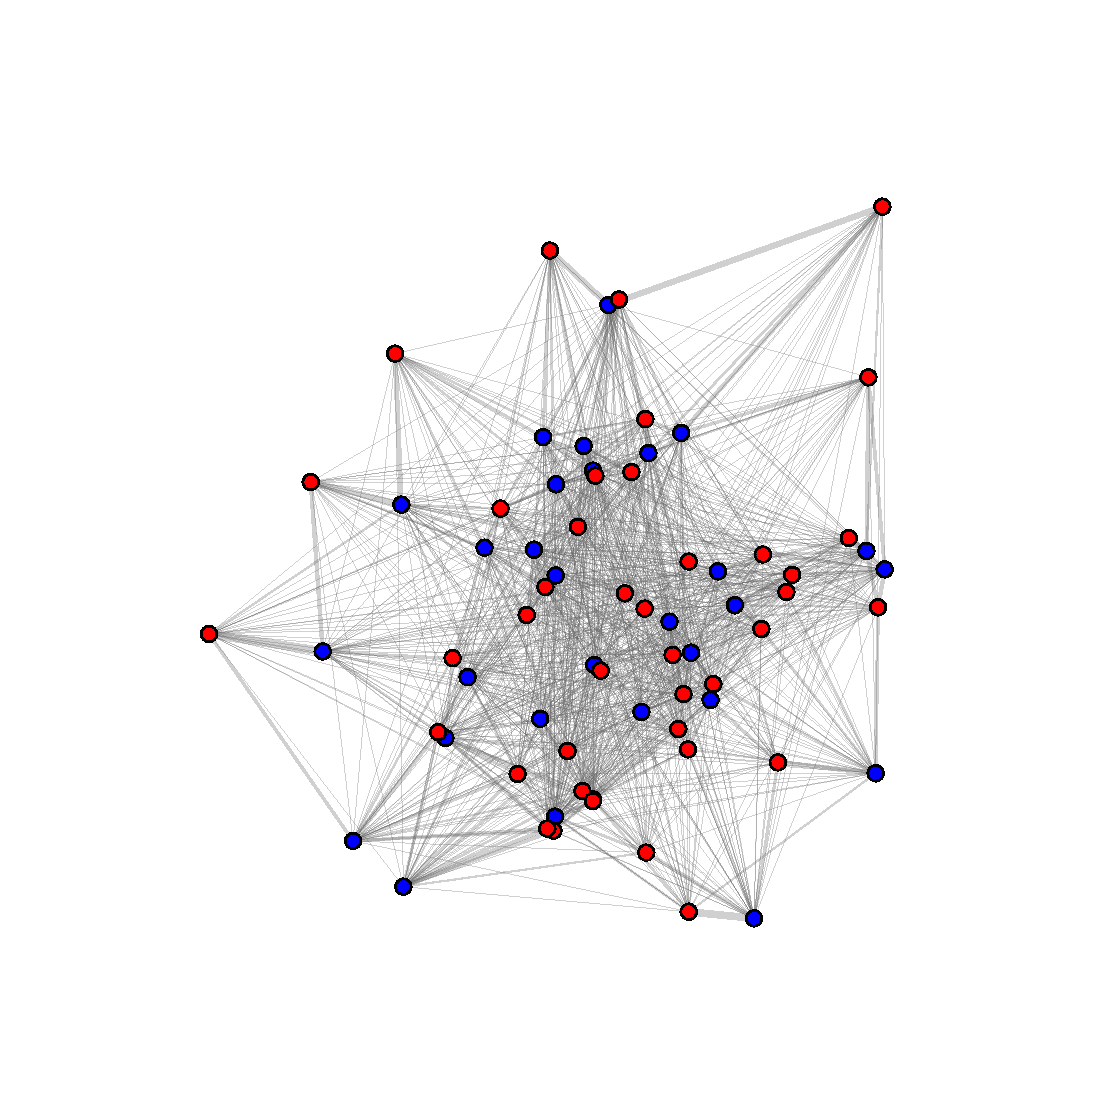
\includegraphics[width=0.24\textwidth]{images/discrete_sinkhorn_graph1}
          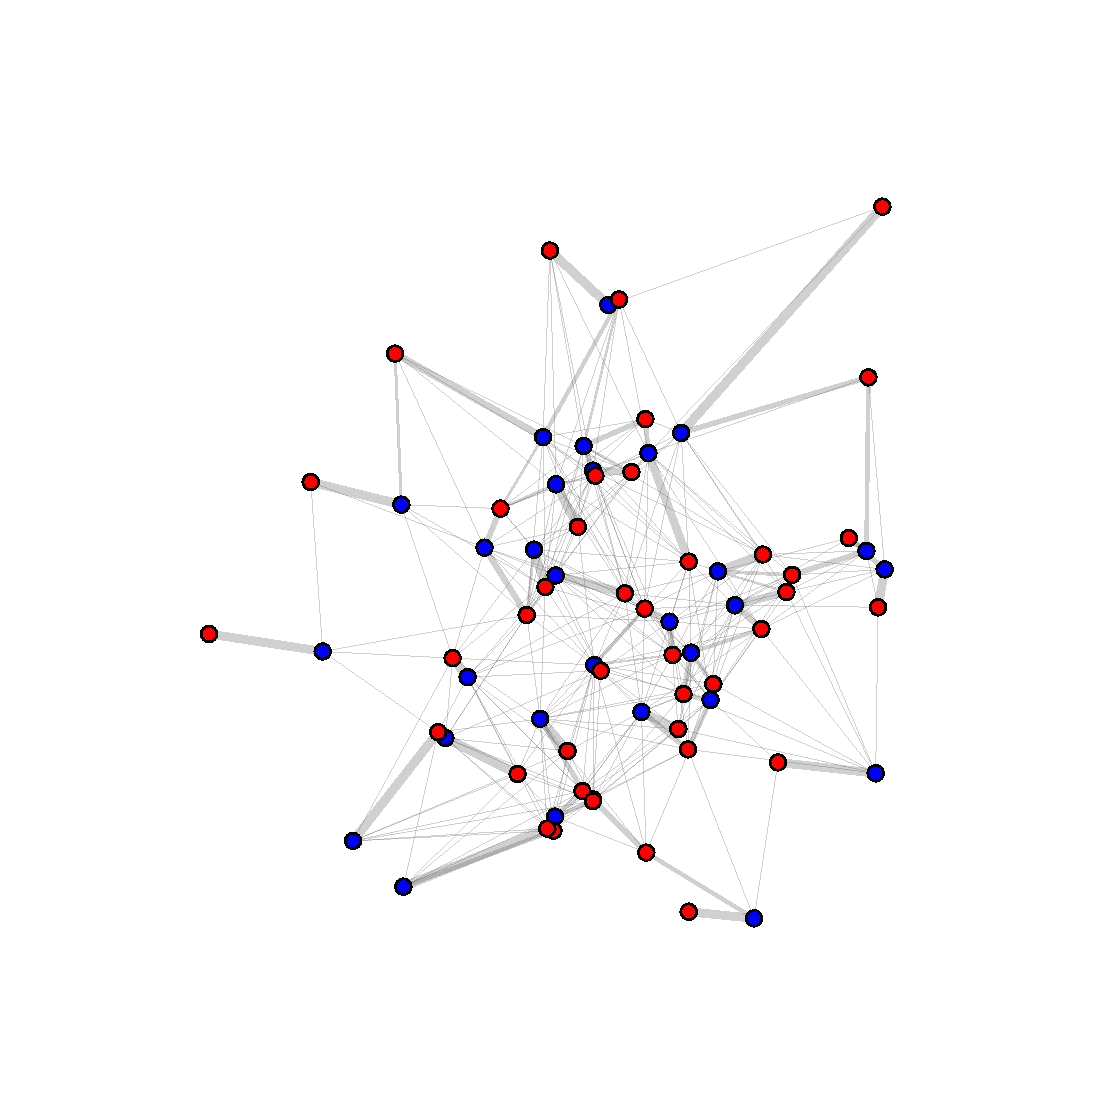
\includegraphics[width=0.24\textwidth]{images/discrete_sinkhorn_graph0.01}
          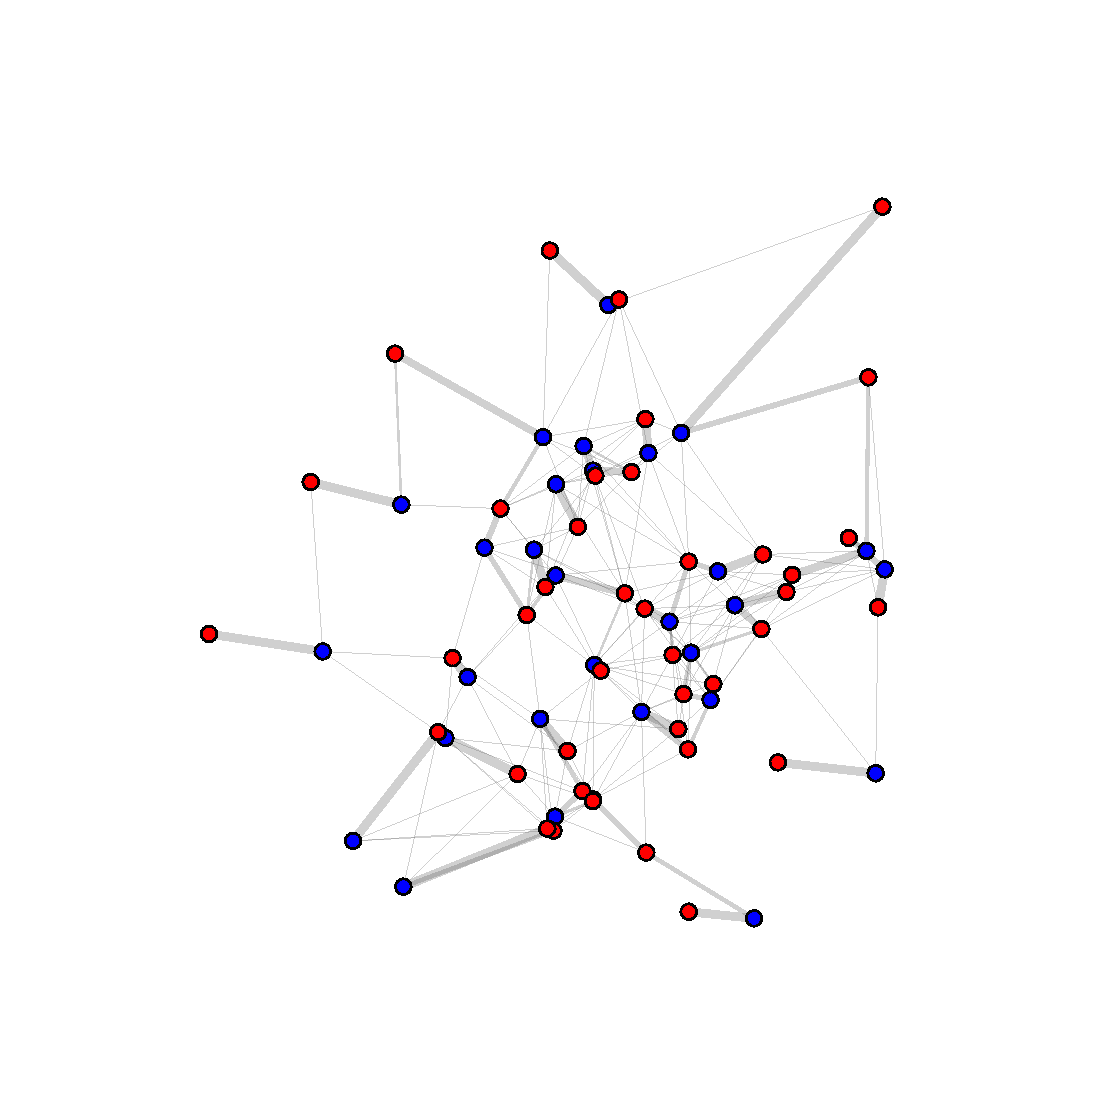
\includegraphics[width=0.24\textwidth]{images/discrete_sinkhorn_graph0.005}
          \caption{Solución del problema entrópico discreto para $\epsilon\in\{1, 0.01, 0.005\}$ (descendente hacia la derecha).}
        \end{figure}

        Esta regularización soluciona los problemas mencionados anteriormente y se puede probar que cuando $\epsilon\to0$, su solución converge a la solución de \eqref{eq:kantorovich} de máxima entropía. Además, esta regularización \textbf{vuelve al problema de Kantorovich diferenciable}, pudiendo ser resuelto usando redes neuronales.

      \end{block}

      \begin{block}{Formulación dinámica y problema del puente de Schrödinger}

        El problema de Kantorovich regularizado resulta ser equivalente al \textbf{problema de Schrödinger estático}, el cual busca un coupling $\pi\in\Pi(\mu,\nu)$ que esté lo más cercano posible (en el sentido de la entropía relativa) a una medida de referencia $\mathcal{W}\in\probmeasure{\xspace\times\xspace}$:

        \begin{equation*}
          \argmin_{\pi\in\Pi(\mu,\nu)} \KL{\pi}{\mathcal{W}}
        \end{equation*}

        Este problema puede ser extendido a una versión dinámica, donde en vez de buscar un coupling $\pi^*$, se busca un proceso estocástico $\mathbb{P}$ (en un horizonte temporal $t\in[0,1]$) que sea lo más similar a un proceso estocástico de referencia $\mathbb{W}$ (usualmente un movimiento browniano). Denotando por $\mathcal{F}(\mu,\nu)$ al conjunto de procesos estocásticos cuyas distribuciones marginales en $t=0$ y $t=1$ son $\mu$ y $\nu$ respectivamente, se puede demostrar que la solución $\mathbb{P}^*$ de este problema dinámico, conocida como \textbf{puente de Schrödinger}, corresponde a interpolar un puente browniano de acuerdo a $\pi^*$:

        \begin{equation*}
          \mathbb{P}^* = \argmin_{\mathbb{P}\in\mathcal{F}(\mu,\nu)} \KL{\mathbb{P}}{\mathbb{W}} \implies \mathbb{P}^*(\cdot) = \int_{\xspace\times\xspace}\mathbb{W}_{xy}(\cdot) \d\pi^*(x,y)
        \end{equation*}

        donde $\mathbb{W}_{xy}$ es un movimiento browniano que empieza en $x$ (para $t=0$) y termina en $y$ (para $t=1$). En la Figura 5 se muestra un ejemplo de este problema dinámico.

        \begin{figure}
          \centering
          \includegraphics[width=0.49\textwidth]{images/sbp_solution0.1}
          \caption{Puente de Schrödinger entre dos distribuciones discretas cuando se considera un proceso de referencia browniano con difusividad $\epsilon=0.1$.}
        \end{figure}

        El problema de Schrödinger también se puede estudiar desde la perspectiva del \textbf{control óptimo}, donde se obtiene una problema de control que generaliza la \textbf{formulación de Benamou-Brenier} del transporte óptimo no regularizado. Además, es posible trabajar directamente con las SDEs que modelan los procesos estocásticos $\mathbb{P}$ y $\mathbb{R}$, donde el término de drift de $\mathbb{P}$ puede ser encontrado resolviendo un sistema acoplado de PDEs. Además, la SDE asociada a $\mathbb{P}$ tiene la misma forma que el proceso reverso de un modelo de difusión basado en SDEs (ver Figura 1), mostrando que los modelos de difusión son un caso particular del problema del puente de Schrödinger.

      \end{block}

    \end{column}
    \separatorcolumn

  \end{columns}
\end{frame}

\end{document}
